\documentclass{acmsiggraph}
\usepackage{mathptmx}
\usepackage{graphicx}

\usepackage{parskip}

%%% short abstract
% By treating an image as a two-dimensional histogram, density-field
% data sets such as those created by chaotic maps can be visualized
% much more effectively and at interactive speeds.

\onlineid{poster\_0071}

\acmformat{print}

\title{Mapping Chaos (poster\_0071)}
\author{
  David Trowbridge\thanks{e-mail: trowbrds@cs.colorado.edu}
\and
  Micah Dowty\thanks{e-mail: micah@navi.cx}
}

\keywords{iterated function systems, chaotic maps, high dynamic range, animation}

\begin{document}

\maketitle

% general background - history of IFSes, etc
\copyrightspace


Iterated Function Systems are a celebrated class of dynamical systems in the
computer graphics world. By defining a constrictive set of functions and
recursing, beautiful fractal images can be created. Classically, these
systems use a set of affine transformations, such as Sierpinski's Gasket.
The addition of nonlinear transformations creates the popular ``flame''
fractal. However, most of these techniques still are based fundamentally
on topology-preserving transformation. If this technique is exapanded to
incorporate space-folding transformations, the function systems can be
simplified to a single map, producing visually coherent images.

Chaotic maps can be thought of as a subclass of Iterated Function Systems.
Whereas traditional iterated function systems use a set equation to create
a tree structure, chaotic maps iterate a single equation. This creates a
single reproducable orbit through the space occupied by the attractor. As
the point jumps around it exposes itself onto the image region, leaving
a characteristic picture of the map.

% techniques
% this should talk about the techniques we used - chaotic maps, stochastic
% noise distributions, histogram imaging, HDR processing, density field stuff,
% that crazy crazy color vector, etc
Although our software has been tested with several maps, we focus on one
attributed to Peter de Jong:
\begin{eqnarray*}
  x_{n+1} &= \sin (a y_n) - \cos (b x_n) \\
  y_{n+1} &= \sin (c x_n) - \cos (d y_n)
\end{eqnarray*}
The initial conditions $x_0$ and $y_0$ are random. For the vast majority
of cases, these chaotic maps contain only one strange attractor. No matter
what initial conditions are chosen, the image will converge towards a
portrait of that attractor. While there are many maps that behave
chaotically, those that involve transcendental functions like the Peter
de Jong map tend to create the most visually interesting attractors.

Generally the literature discussing these maps is full of black and white
images, created where each pixel is blackened as the point $(x_n, y_n)$
moves around the image region. This technique is often sufficient for
analyzing the structure of a map but does not provide a sound basis for
the use of the map as an artistic entity. The structure of the attractor
is only minimally visible using such techniques, because a long iteration
run will quickly result in a completely black image.

Instead, the entire image region is treated as a two dimensional histogram.
Unlike previous techniques, where each $x_n$ and $y_n$ plotted by darkening a
a pixel directly, this histogram technique maintains total image intensity as
more iterations are performed. As more samples accumulate in the histogram,
the image simply gets more detailed. Instead of an image containing only a
few thousand iterations of the map, millions or billions of points can be
plotted with no loss of detail.

\begin{figure}[ht]
\centering
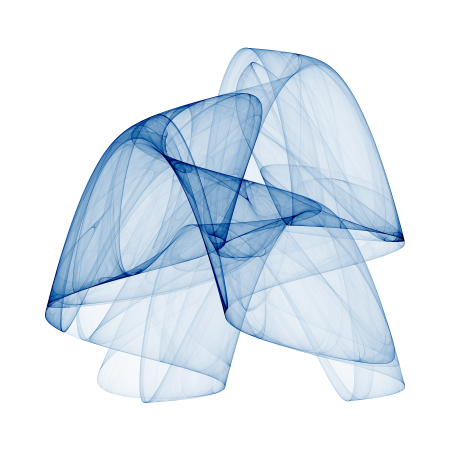
\includegraphics[width=1.5in]{1.png}
\caption{A Typical Attractor.}
\end{figure}

Like other rendering techniques that progressively refine an image, this
histogram method performes particularly well in interactive applications.
Our software for interactively browsing parameter space runs iterations
for each frame only until a predetermined amount of time has elapsed,
displaying a low quality but complete image nearly instantaneously.
Instead of waiting for a preset number of iterations to complete, the user
can zoom through parameter space quickly, viewing only what the CPU has time
to render. As soon as the user stops changing parameters, the image quality
will begin to improve.


% possible applications
% hrm...screensavers? textures? it's...art! really!
blar blar blar blar blar blar blar blar blar blar blar blar blar blar blar
blar blar blar blar blar blar blar blar blar blar blar blar blar blar blar
blar blar blar blar blar blar blar blar blar blar blar blar blar blar blar
blar blar blar blar blar blar blar blar blar blar blar blar blar blar blar
blar blar blar blar blar blar blar blar blar blar blar blar blar blar blar
blar blar blar blar blar blar blar blar blar blar blar blar blar blar blar
blar blar blar blar blar blar blar blar blar blar blar blar blar blar blar
blar blar blar blar blar blar blar blar blar blar blar blar blar blar blar

% future work
% spline-based interpolation through parameter space, automatic evasion
% of fixed-points and limit cycles.

blar blar blar blar blar blar blar blar blar blar blar blar blar blar blar
blar blar blar blar blar blar blar blar blar blar blar blar blar blar blar
blar blar blar blar blar blar blar blar blar blar blar blar blar blar blar
blar blar blar blar blar blar blar blar blar blar blar blar blar blar blar
blar blar blar blar blar blar blar blar blar blar blar blar blar blar blar
blar blar blar blar blar blar blar blar blar blar blar blar blar blar blar
blar blar blar blar blar blar blar blar blar blar blar blar blar blar blar
blar blar blar blar blar blar blar blar blar blar blar blar blar blar blar

\end{document}
